% !TeX root = ../main.tex

\chapter{绪论}

\section{系统开发背景}
进入21世纪以后,各国都在积极发展信息安全技术,同时由于知识经济以及人工智能、全球互联时代的到来,集成电路产业在国民经济中发挥着越来越不可替代的作用。我国的集成电路产业经过了几十年的发展,在某些应用领域也取得了不错的成绩,但在高性能处理器以及芯片设计的关键技术中,仍然面临着巨大的挑战。此外,我国的集成电路产业发展还承担着许多来自国际的压力\cite{huzhenbo,huzhenbo1}。不管是2018年中美贸易战中“中兴事件”和“华为事件”的发生,还是其他大国对我国实行的禁运政策,都让我国在市场竞争竞争中处于下风。


作为软硬件之间至关重要的接口,指令集架构(Instruction Set Architecture, ISA)是处理器的灵魂。作为一款完全开源的指令集架构,RISC-V在众多指令集架构中脱颖而出,不仅是因为其后发优势,提出模块化设计的概念,而且因为它开放,包容,提供了高度灵活的配置空间,在积极拥抱开源软件的今天,RISC-V已经成为未来的主流架构,而随着RISC-V开源社区的日益壮大,更多的芯片设计厂商选择RISC-V作为其指令集架构,指导芯片的设计生产.在集成度越来越高的今天,面对数千万乃至上亿晶体管的规模,那种“设计硬件原型-实现-评估-改进-再实现”的模式已经无法满足现代设计应用的需求\cite{jichengdu}.研究表明,如果在CPU的方案论证和设计阶段,没有及时发现问题与瓶颈,将会使后续的工作变得更为困难且代价更加高昂。因此,在开发一个新的体系结构处理器时,为了确保处理器功能特性和性能参数达到设计的预期目标,对体系结构进行验证是一个必不可少的步骤\cite{buzhou}.除此之外,在芯片开发后期,软硬件适配工作作为测试的重点,往往也需要模拟器环境的支持,厂商可以根据自身产品特性,设计相应的模拟器,并在此基础之上进行软件移植工作和前期软硬件设配工作,以此来提高芯片验证与测试工作的效率。当前RISC-V的软件生态尚不完善,各种软件的RISC-V移植工作正在开源社区如火如荼地进行中,对于芯片设计和开发厂商,更加需要积极地参与进来,RISC-V架构的体系结构模拟器将在此类工作中扮演重要的角色.



\section{国内外发展现状}
龙芯中科技术有限公司在使用模拟器辅助处理器设计的文献中提到\cite{zhang2007sim,gao2007simos},在龙芯2号处理器研发的早期,开发了模拟器ICT-Godson,由于该模拟器对硬件模拟过于详细,导致其速度和灵活性不足.因此,龙芯基于开源模拟器Simple-Scalar\cite{austin2002simplescalar}重新设计实现了Sim-Godson模拟器\cite{zhang2007sim}.和ICT-Godson模拟器相比,Sim-Godson运行速度更快、灵活性更高,并且支持大程序评估\cite{zhang2007sim}.Sim-Godson可以支持时序模拟和功能模拟,可以直接加载二进制可执行程序进行模拟,该模拟器主要用于处理器核的微结构性能探索.
虽然借用了Simple-Scalar的基础模块,但Sim-Godson对其进行了大量修改定制,使其能够高精准地对龙芯2号处理器核微结构进行模拟.基于Simple-Scalar中自带的指令集仿真器和I/O仿真器进行执行加速,其速度可以达到0.5MIPS(million instructions per second).经过详细校准,Sim-Godson模拟器与ICT-Godson的误差平均不到5\%\cite{zhang2007sim}.类似地,基于Simple-Scalar进行二次开发的模拟器还有Sim-alpha\cite{desikan2001sim}.


IBM于2012年某研讨会中做了题为“IBM使用模拟器的经验”的报告\cite{kistlerexperiences},对于IBM如何在处理器设计过程中使用模拟器进行了介绍.在处理器前期地设计规划时期,IBM使用Mambo\cite{boh}模拟器的时钟精确模式进行微结构探索和粗粒度微结构定义.Mambo模拟器对微结构主要模块和结构进行了模拟,该阶段Mambo由踪迹(trace)驱动,主要运行和研究用户态应用,对处理器的产品竞争力进行横向比较研究\cite{kistlerexperiences}.在微结构设计实现期间,IBM使用基于公司内部专用“T”语言编写的时钟精准模拟器M1进行详细模拟处理器微结构\cite{kistlerexperiences},如图~\ref{fig:IBM}所示.M1是以Mambo模拟器或者硬件上抓取的踪迹作为输入,并且可以收集非常详细的微结构数据进行性能评估.
\begin{figure}[h]
  \centering
  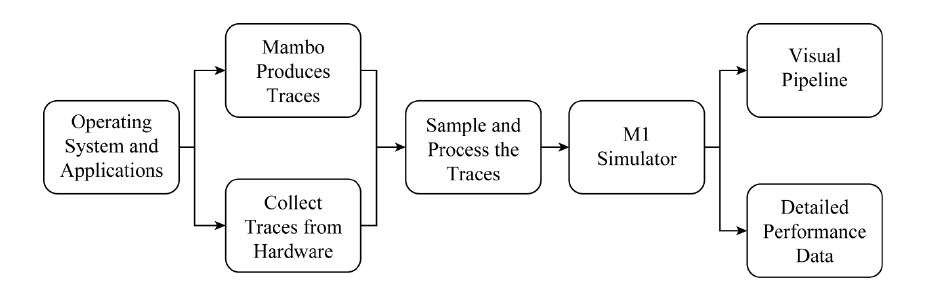
\includegraphics[width=1.0\textwidth]{IBM.png}
  \caption{IBM模拟器框架}
  \label{fig:IBM}
\end{figure}  


为了加速M1模拟器的执行速度,需要对所抓取的踪迹进行取样,同时为了方便调试,M1支持微结构性能数据可视化功能.在处理器验证阶段,IBM使用Mambo作为处理器验证参考模型辅助进行验证,此阶段Mambo可以为处理器功能正确性提供参考结果.Mambo模拟了所有处理器的功能特征,把某些性能相关的微结构维护操作(例如cache维护类指令)翻译成空(nop)操作,对于计算类指令产生准确的结果,并精准追踪处理器寄存器的状态变化,同时支持指令撤销操作,为处理器验证提供参考.IBM基于Mambo模拟器曾发现PowerPC CPU的一个控制寄存器存在竞争条件,使得该设计错误在流片之前就被发现并修改.在该阶段,IBM还使用自研的由多个FPGA(field programmable gate array)组成的VHDL(very-high-speed integrated circuithardware description language)仿真加速器Twinstar\cite{asaad2012cycle}进行处理器综合验证.Twinstar是时钟精准的仿真加速器,其推进方式是事件驱动模式,可以对整个处理器芯片进行仿真,以二进制程序作为输入,还支持详细的指令踪迹和处理器状态的实时追踪.该平台运行速度可以达到4MHz并可以运行未经修改的系统软件.类似Twinstar的验证平台还有帕拉丁\cite{chaix2019implementation}等.
在系统软件开发方面,IBM基于Mambo(加速模式),Simics\cite{magnusson2002simics},BGLsim\cite{ceze2003full}等多种平台,在流片之前就开始进行固件、操作系统、虚拟机管理器等软件的早期开发.IBM基于Mambo模拟器曾开发了K42操作系统,在芯片可用之后1周内就启动了操作系统\cite{boh}.IBM基于BGLsim-multi\cite{ceze2003full}平台和基于OMNeT++\cite{varga2010omnet}开发的MARS(message passing interface application replay simulation)模拟平台还可以对机群网络相关的功能进行模拟,模拟器由可执行程序或者踪迹驱动,其中MARS平台还可以对MPI(message passing interface)类应用进行调优.


此外,比较著名的研究项目还有法国的嵌入式多体系结构模拟器Qemu\cite{bellard2005qemu}、上海同济大学研制的PEMU\cite{huang}以及浙江大学开发的WuKong系统\cite{wukong}等。


\section{本文主要工作}
为了加快芯片开发项目中的系统软件开发过程,以及辅助进行处理器验证,本文从真实的芯片开发项目工作流程入手,设计并实现了一款针对RISC-V体系结构的指令集功能模拟器,可以使得芯片开发团队脱离硬件平台进行并发的系统软件移植/开发/测试工作,提供对真实硬件的功能模拟,以及丰富的调试手段,缩短软件开发周期,辅助处理器验证工作.主要完成的工作如下:


(1)参照RISC-V用户手册,特权级架构手册,以及实际的硬件设计方案,对RISC-V标准拓展指令集共196条汇编指令进行C++功能函数模拟,其中大部分指令功能可以直接由RISC-V指令集手册获取,少部分指令(主要是特权架构指令)参照硬件设计团队具体的chisel代码进行翻译,对硬件设计的功能框架进行建模,确定模拟器的实现方案,规划具体功能模块的边界.


(2)实现RISC-V指令集模拟器前后端模块,添加丰富的调试手段,设计并实现平台级中断控制器PLIC和部分外设模拟,可以直接在模拟器进行外设驱动的开发,结合实际项目需求,添加UI可视化界面,进一步加强模拟器的易用性.在实际的芯片开发项目中帮助团队进行系统软件开发工作,并对处理器进行辅助验证.


本人负责的主要工作有进行指令集模块的功能函数设计实现,模拟器后端整体框架的搭建,平台级中断控制器的功能建模与实现,调试交互模块的可视化界面优化,以及测试模拟器是否符合设计需要.


\section{论文的组织结构}
本论文总共分为7章,各章节内容安排如下:


第一章:绪论。本章首先简要介绍了RISC-V指令集架构和体系结构模拟器的背景,然后对国内外主要体系结构模拟器进行举例分析,进而确定了本模拟器的设计思路,最后阐述了本文的主要工作以及论文的组织结构。
第二章:相关技术分析。本章对体系结构模拟器的各种技术知识进行分析,包括体系结构各类别和作用,以及指令集模拟策略等相关技术,然后针对RISC-V指令集架构特性,确定了基于解释型的模拟策略作为本模拟器的设计方案.
第三章:系统需求分析。本章主要是采用面向对象分析的方法对模拟器用户的需求进行分析与建模,明确模拟器的功能需求和性能需求,建立系统需求规格说明书。
第四章:系统概要设计。本章主要是对RISC-V指令集模拟器的总体框架进行设计与描述,包括系统的静态软件结构、动态运行流程,确立了模拟器的四个功能模块:指令集模块,CPU和总线模块,中断模块以及调试交互模块。
第五章:系统详细设计与实现。本章主要是对RISC-V指令集模拟器的各个功能模块的具体实现进行阐述,确定每个模块的功能边界、数据结构和接口细节,并进行具体实现。
第六章:系统测试与结果分析。本章主要是对RISC-V指令集模拟器进行单元测试、配置项测试和系统测试,包括测试需求分析和测试用例设计的过程,并依据测试结果,分析模拟器功能和性能的实现情况。
第七章:结论与期望。本章对全文工作进行总结,简要地回顾了RISC-V指令集模拟器的开发背景,介绍了系统的具体设计与实现情况,并指出了当前系统所存在的问题以及未来可能进行改进的方向。


